\documentclass{standalone}

\usepackage{pgfplots}
\usepackage{tikz}
\usetikzlibrary{shapes,arrows,positioning}

% Tikzstyles and commands
\tikzstyle{decision} = [diamond, aspect=2, draw, fill=green!20, minimum size=7mm, node distance=2cm]
\tikzstyle{block} = [rectangle, draw, fill=blue!20, minimum size=7mm, node distance=1.5cm]
\tikzstyle{arrow} = [draw, thick, color=black!50, ->]
\tikzstyle{line} = [draw, thick, color=black!50, -]
\tikzstyle{cloud} = [draw, ellipse,fill=red!20, minimum size=7mm, node distance=1.5cm]
\tikzstyle{answer}=[near start,color=black]
\tikzstyle{fake}=[inner sep=0cm, line width=0mm, fill=black!50, radius={\pgflinewidth}]
\tikzstyle{point}=[inner sep=0.5mm, line width=0mm, shape=circle]

\begin{document}

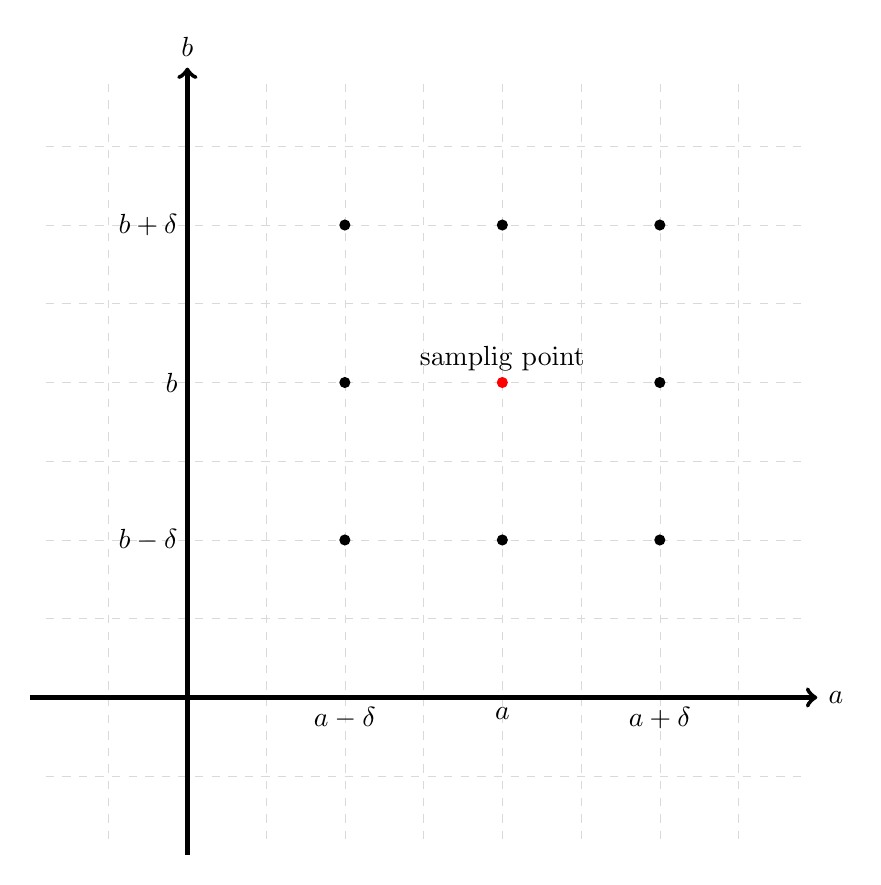
\begin{tikzpicture} [x=2cm, y=2cm]


  \draw[help lines, color=gray!30, dashed] (-0.9,-0.9) grid (3.9,3.9);
  \draw[->,ultra thick] (-1,0)--(4,0) node[right]{$a$};
  \draw[->,ultra thick] (0,-1)--(0,4) node[above]{$b$};

  \node[point, fill=black] at (1,1) {};
  \node[point, fill=black] at (1,2) {};
  \node[point, fill=black] at (1,3) {};
  \node[point, fill=black] at (2,1) {};
  \node[point, fill=red] (sampoint) at (2,2) {};
  \node[point, fill=black] at (2,3) {};
  \node[point, fill=black] at (3,1) {};
  \node[point, fill=black] at (3,2) {};
  \node[point, fill=black] at (3,3) {};

  \node[above of=sampoint, node distance=3mm, inner sep=0cm] {samplig point};

  \node[below] at (1,0) {$a-\delta$};
  \node[below] at (2,0) {$a$};
  \node[below] at (3,0) {$a+\delta$};
  \node[left] at (0,1) {$b-\delta$};
  \node[left] at (0,2) {$b$};
  \node[left] at (0,3) {$b+\delta$};

\end{tikzpicture}

\end{document}
